\section{Data assimilation}

\subsection{Introduction}
\noindent Data assimilation is nowadays widely used to make predictions in complex systems, for example in weather forecasting or ocean simulation. Data assimilation is a method that combines observations with the output of a model to improve a prediction. 
The main idea is to combine information from our model and from observations, in order to have a more reliable analysis. Sometimes what you are trying to improve in our model may not be in the same space as what our observe this is something that we need to consider while doing our assimilation. It is also important to control our output, it is up to us to decide which input is responsible for the error in our output. This means that there will be uncertainties coming from the model or from the observations, these uncertainties coming from our input will also translate into uncertainties in our output.
At the end of the data assimilation we will obtain an output which will be an estimate of the unknown quantity process the state variables.
The best estimate is searched for as a linear combination of the background estimate and the observations:

$$x^a=Lx^b+Ky^0$$


\noindent Data assimilation methods are often split into two families: statistical methods and a variational methods.
The second one, called variational methods, consists in minimizing a cost function.
\subsection{statistical approach}
\subsubsection{Kalman filter}
The Kalman filter method consists in looking for $x^a$ an analysis, this analysis will be a linear combination of what we already know, our model and our observations.
To explain this method let's consider that we observe a single quantity, an estimation of a scalar quantity at a point in space. For example we are observing the temperature in the middle of the room, and the model also simulate the temperature in the middle of the room.  We will then have :
$$x^a=x^b+K(y-x^b)$$
with $x^a=\begin{pmatrix}
 x_1^a  \\ 
 \vdots \\
 x_n^a \\
\end{pmatrix}$ the analysis, $x^b=\begin{pmatrix}
 x_1^b  \\ 
 \vdots \\
 x_n^b \\
 \end{pmatrix}$ the background or model, $y=\begin{pmatrix}
 y_1  \\ 
 \vdots \\
 y_p \\
 \end{pmatrix}$ the observation and $K$ the gain matrix of size $p \times p$. 

\noindent To simplify the redaction let's consider that we are trying to find the true state of a single point(1D),we suppose that the true state $x^t$ exists so:
$$x^a-x^t=x^b-x^t+K(y-x^t-x^b+x^t).$$
Let's define the errors:
$$\begin{aligned}
&\epsilon^a=x^a-x^t, \\
&\epsilon^b=x^b-x^t, \\
&\epsilon^y=y-x^t, \\
\end{aligned}$$
So we will have:
$$\epsilon^a=\epsilon^b+K(\epsilon^y-\epsilon^b)$$
If we have many realisation of these error, then we can write:
$$<\epsilon^a>=<\epsilon^b>+K(<\epsilon^y>-<\epsilon^b>)$$
We want to have the analysis error variance as low as possible .So we want to minimize $<(\epsilon^a)^2>$ with respect to $K$ ,this will give us:
$$<(\epsilon^a)^2>=<(\epsilon^b)^2>+K^2<(\epsilon^y-\epsilon^b)^2>+2K<\epsilon^b(\epsilon^y-\epsilon^b)^2>$$
$$2K<(\epsilon^y)^2+(\epsilon^b)^2>-2<(\epsilon^b)^2>=0$$
\noindent We assume that the errors in the background and observation are uncorrelated.
$$K=\frac{<(\epsilon^b)^2>}{<(\epsilon^b)^2>+<(\epsilon^y)^2>} \Rightarrow K=\frac{(\sigma^b)^2}{(\sigma^b)^2+(\sigma^y)^2} $$
where $(\sigma^y)^2$ is the observation error variance and $(\sigma^b)^2$ is the background or model error variance.
\newline\noindent If we have $(\sigma^y)^2=0$, $K=1$ and $x^a=y$  this means that the observation are perfect.
\newline\noindent And if $(\sigma^b)^2=0$, $K=0$ and $x^a=x^b$ this is equivalent to ignoring the observations.
\vspace*{5mm}
\newline Now that we have explained the method for finding $x^a$ let's try to generalize our formula in a multi-dimensional case.

$$\left\{\begin{aligned}
		&x^a=(I-KH)x^b+Ky^0=x^b+K(y^0-H(x^b)) \\
        &K=BH^T(HBH^T+R)^{-1} \\
	\end{aligned}\right.$$
With $K$ the gain or weight matrix, $(y^0-H(x^b))$ the innovation and $H$ the linear model of the observations.
This formulation is called the Best Linear Unbiased Estimator (BLUE) or least squares analysis.
The principle of the Kalman filter is based on this formulation. Here is a small figure which illustrates the Kalman filter.
\vspace*{5mm}
\begin{figure}[H]
    \centering
		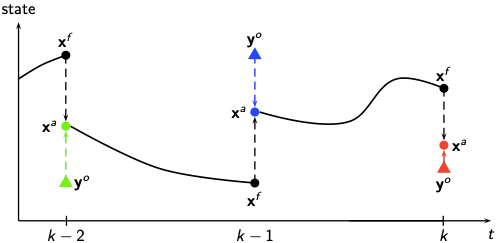
\includegraphics[width=0.8\textwidth]{"images/enkf/schema_kalman_filter.png"}
	\caption{Kalman filter}
\end{figure}
The general idea consists in estimating the state at time $k$ from an estimate at time $k-1$ and measurements at time $k$.
We do the estimation in two steps:
\begin{enumerate}[label=\textbullet]
		\item Prediction of the state from the evolution model
		\item Correction of the prediction from the measurements
	\end{enumerate}

\subsubsection{Kalman filter algorithm}
Let us precise the notations we will use:

\noindent $k\in \mathbf{N}$, $x_k^f ,x_k^a\in \mathbf{R^n}$ and $P_k^f,P_k^a \in \mathbf{R^{n\times n}}$:
 \begin{enumerate}[label=\textbullet]
		\item $k$ time index
		\item $x_{k}^{f}$ forecast state (background), forecast error covariance matrix $P_{k}^{f}$
		\item $x_{k}^{a}$ analyzed state (result of the assimilation process), analysis error covariance matrix $P_{k}^{a}$
	\end{enumerate}
\noindent Operators:
    \begin{enumerate}[label=\textbullet]
		\item model operator $ M_{k,k+1}(x_{k}^{t}) $ model error $\eta
		_{k,k+1}$, covariance matrix $Q_k$
		\item observation operator $ H_k (x^t ) $ , observation error $\epsilon^0$, covariance matrix $R_k$
	\end{enumerate}
\noindent The hypotheses necessary for the application of the Kalman filter are:
    \begin{enumerate}[label=\textbullet]
		\item Model and observations operators $M_{k,k+1}$ and $H_k$ are linear.
		\item Errors are unbiased, Gaussian, independent and white in time for example for the observation we will have $<\epsilon_k^0\epsilon_j^{0T}>=0$ if $k\ne j$:.
	\end{enumerate}
So finally we obtain the Kalman filter algorithm.
\begin{enumerate}[label=(\roman*)]
\item Initialization: $x_0^f$ and $P_0^f$ are given, equal to $x^b$ and $B$
\item BLUE:
$$\begin{aligned} &K_k=(H_kP_k^f)^T[H_k(H_kP_k^f)^T+R_k]^{-1} \\
&x_k^a=x_k^f+K_k(y_k^0-H_kx_k^f) \\
&P_k^a=(I-K_kH_k)P_k^f \\
\end{aligned}$$
\item Forecast step:
$$\begin{aligned} 
&x_{k+1}^f=M_{k,k+1}x_k^a \\
&P_{k+1}^f=M_{k,k+1}P_k^aM_{k,k+1}^T+Q_k\\
\end{aligned}$$
\end{enumerate}



\subsection{Variational approach}
\subsubsection{Minimizing a cost function}
\noindent In the previous part we have seen that there is a method called Kalman filter whose purpose is to make prediction with a model and observations, but there is also an other method to make data assimilation like the variational assimilation, which solves the analysis problem through an optimisation (minimisation of a cost-function). This allows to solve the global problem in one go, and it is now widely used in the meteorological community. So variational data assimilation methods lead to the minimization of a cost function involving quadratic forms based on the both the background and observation covariance matrices. When the observation operator is linear the formulation of the cost function leads to the best the Best Linear Unbiased Estimation. An alternative way to define the analysis is to consider it as the maximum of the a posteriori p.d.f of the state given the observation and the background:
$$x^a=\arg\max_{x}p(x|y ~ , ~ x^b)$$
Using bayesian approach $p(x|y)~\alpha~ p(y|x)p(x)$ we can simplify our probability by:
$$p(x|y ~ , ~ x^b)=\frac{p(y ~ , ~ x^b| x)p(x)}{p(y ~ , ~ x^b)}$$
We assume that observation and background errors are uncorrelated so we will have then:
$$(x|y ~ , ~ x^b)=p(y|x)p(x^b|x)$$
So we can define the cost function as:
$$J(x)=-log(p(y|x)p(x^b|x)+cst \\
=-log(p(y|x))-log(p(x^b|x))+cst$$
We can find the analysis by solving a minimization problem:
$$x^a=\arg\min_{x}J(x)$$
We assume that p.d.f are Gaussian.
$$p(x^b|x)=(2\pi)^{-n/2}|B|^{-1/2}\exp({-\frac{1}{2}(x-x^b})^TB^{-1}(x-x^b))$$
$$p(y|x)=(2\pi)^{-m/2}|R|^{-1/2}\exp({-\frac{1}{2}(y-H(x)})^TR^{-1}(y-H(x)))$$
Which will lead us to:
$$J(x)=\frac{1}{2}(x^b-x)^TB^{-1}(x^b-x)+\frac{1}{2}(y-H(x))^TR^{-1}(y-H(x))$$
This is called the cost function of 3D-Var Approach.
\subsubsection{Generalisation of the 3D-Var Approach}
\noindent Let's go back to the notations:
\noindent  $x^b ,x^a\in \mathbf{R^n}$,$y^0 \in \mathbf{R^m} $ and $B \in \mathbf{R^{n\times n}}$:
 \begin{enumerate}[label=\textbullet]
		\item $x$ state vector or input parameters
		\item $x^{b}$ background state (a priori information), background  error $\epsilon^b=x^b-x^t$ covariance matrix $B$
		\item $x^{a}$ analyzed state (result of the assimilation process)
		\item $y^0$ observation vector
	\end{enumerate}
\noindent Operators:
    \begin{enumerate}[label=\textbullet]
		\item model operator $M_{0 \rightarrow k}(x_0^t)$
		\item observation operator $H_k(x^t)$ observation error $\epsilon_k^0$, covariance matrix $R_k$
	\end{enumerate}
\noindent Variational approach of BLUE consists in finding $x^a=\arg\min_{x}J$:
$$\begin{aligned}
J(x)&=\frac{1}{2}(x^b-x)^TB^{-1}(x^b-x)+\frac{1}{2}(y-H(x))^TR^{-1}(y-H(x)) \\
&=\frac{1}{2}\|x-x^b\|_B^2+\frac{1}{2}\|H(x)-y^0\|_R^2
\end{aligned}$$
If the problem is time-dependent, and the unknown x is the initial state vector:
$$\begin{aligned}
J(x)&=\frac{1}{2}\|x-x^b\|_B^2+\frac{1}{2}\|H_k(x)-y_k^0\|_{R_{k}}^2 \\
&=\frac{1}{2}\|x-x^b\|_B^2+\frac{1}{2}\|H_k(M_{0 \rightarrow k}(x))-y_k^0\|_{R_{k}}^2
\end{aligned}$$
with:
$$\begin{aligned}
J^b&=\frac{1}{2}\|x-x^b\|_B^2\\
J^o&=\frac{1}{2}\|H_k(M_{0 \rightarrow k}(x))-y_k^0\|_{R_{k}}^2
\end{aligned}$$
\vspace*{5mm}
Here is a diagram that illustrates the 3D Var method 
\begin{figure}
    \centering
		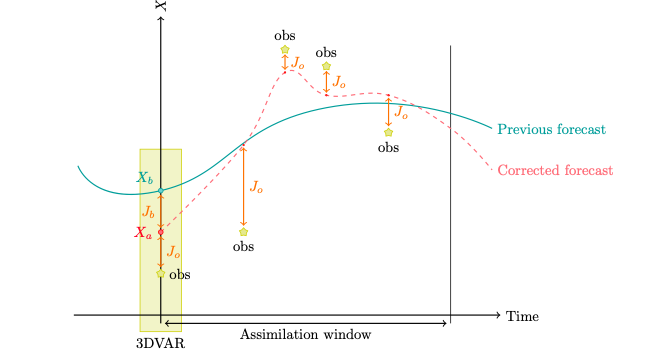
\includegraphics[width=0.8\textwidth]{"images/enkf/schema_3D_Var.png"}
		\caption{3D-Var}
\end{figure}
\subsubsection{From 3DVar to BLUE}
\noindent We have are 3D-Var cost function:
$$J(x)=\frac{1}{2}\|x-x^b\|_B^2+\frac{1}{2}\|H(x)-y\|_{R}^2 $$
 Let us minimize J and compute the variation of $J(x)$ with respect to
a variation of $x$ :
$$\begin{aligned}
\delta J(x)=&\frac{1}{2}(\delta x)^TB^{-1}(x-x^b) \\
&+\frac{1}{2}(x-x^b)^TB^{-1}\delta x \\ &+\frac{1}{2}(-H(\delta x))^TR^{-1}(y-H(x)) \\
&+\frac{1}{2}(x^b-H(x))R^{-1}(-H(\delta x)) \\
=&(\delta x)^TB^{-1}(x-x^b)-(\delta x)^TH^TR^{-1}(y-H(x)) \\
=&(\delta x)^T \nabla J
\end{aligned}$$
The extremum condition is 
$$\nabla J=B^{-1}(x^*-x^b)-H^TR^{-1}(y-Hx^*)=0$$
so we will have:
$$x^*=x^b+(B^{-1}+H^TR^{-1}H)^{-1}H^TR^{-1}(y-Hx^b)$$
Grave to Sherman-Morrison-Woodbury identity,
$$K^*=(B^{-1}+H^TR^{-1}H)^{-1}H^TR^{-1}=BH^T(R+HBH^T)^{-1}$$
Therefore, we have that our solution $x$ of the minimization problem coincides with the BLUE optimal analysis $x^a$
\subsection{Ensemble Kalman Filter}
\noindent We have seen so far two methods to do data assimilation, these methods are valid only for linear systems, but the Lorenz system is non-linear, that's why we will introduce the Ensemble Kalman Filter method which works well for non-linear systems. The ENKF method consists in using the Kalman filter method in high dimension and compare P by a set of states $x_1,x_2,..,x_{m}$. So we can approximate the moments of the error by the moments of the sample.
The we have:
$$x_i^a=x_i^f+K[y-h(x_i^f)]$$
with $h(x_i^f)$ the observation operator.
We can also define the Kalman gains: 
$$K=P^f H^T(HP^f H^T+R)^{-1}$$
To begin with we can estimate the
forecast error covariance matrix as:
$$P^f=\frac{1}{m-1}\sum_{i=1}^{m}(x_i^f-\bar{x}^f)(x_i^f-\bar{x}^f)^T~~with~~\bar{x}^f=\frac{1}{m}\sum_{i=1}^{m}x_i^f .$$ 
\noindent We can factorized the forecast error covariance matrix by:
$$P^f=X_f X_f^T$$
where $X_f$ is an $n \times m$ matrix whose columns are the normalized anomalies or normalized perturbations,
$$[X_f]_i=\frac{x_i^f-\bar{x}^f}{\sqrt{m-1}}$$
In addition, we have:
$$
\bar{x}^a=\frac{1}{m}\sum_{i=1}^mx_i^a~~,~~~~[X_a]_i=\frac{x_i^a-\bar{x}^a}{\sqrt{m-1}} $$
\subsection{Presentation of the results}
\subsubsection{Harmonic oscillator}
\noindent After the implementation for the data assimilation, to test it, the idea was to find an equation for which we know the exact result. That's why we chose to test it with the harmonic oscillator equation:
$$\qquad \frac{\partial x}{\partial t}=v \quad \Rightarrow \quad \frac{\partial^2 x}{\partial t^2}=\frac{\partial v}{\partial t}$$



\noindent For the first case we chose to take a model that will be solved with RK4 and as observation we chose to take the exact solution. We must also choose $P$, $R$ and $Q$ with $Q$ covariance matrix associated with the models, $R$ covariance matrix associated with the observations and $P$ covariance matrix associated with the forecast state.
The observation operator will only take the first value which is $\frac{\partial x}{\partial t}=v$ because we only observe the exact value of $v$ .
\newpage
\noindent Let's take :
\begin{enumerate}[label=\textbullet]
  \item For the initial point: $(x(0),v(0))=(2,0)$ 
  \item For the period : \; $Pe$=$\frac{2\pi}{\omega_0=2}$,\quad $x_0=2$ \quad, $\phi_0=0$ 
  \item For the discretisation $dt$=$\frac{Pe}{20}$, and for the time range :\quad $[t_0,T]=[0,3Pe]$
\end{enumerate}
\noindent\newline Several cases are studied:
\begin{enumerate}[label=\textbullet]
	\item For the first case:
	        $$P=\begin{pmatrix}
            0.01 & 0. \\
            0. & 0.01 \\
            \end{pmatrix} ,
            Q=\begin{pmatrix}
            0.01 & 0.\\
            0. & 0.01 \\
            \end{pmatrix},
            R=\begin{pmatrix}
            0.001 \\
            \end{pmatrix}.$$ 
        \item For the second case:
	        $$P=\begin{pmatrix}
            1. & 0. \\
            0. & 1.\\
            \end{pmatrix} ,
            Q=\begin{pmatrix}
            0.01 & 0.\\
            0. & 0.01 \\
            \end{pmatrix},
            R=\begin{pmatrix}
            0.001 \\
            \end{pmatrix}.$$ 
        \item For the third case:
	        $$P=\begin{pmatrix}
            0. & 0. \\
            0. & 0.\\
            \end{pmatrix} ,
            Q=\begin{pmatrix}
            0. & 0.\\
            0. & 0. \\
            \end{pmatrix},
            R=\begin{pmatrix}
            0.001 \\
            \end{pmatrix}.$$ 
\end{enumerate}
\begin{figure}[H]
    \centering
		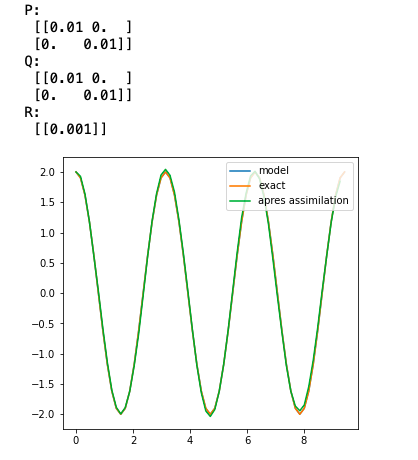
\includegraphics[width=0.4\textwidth]{"images/enkf/oscillator1.png"}
		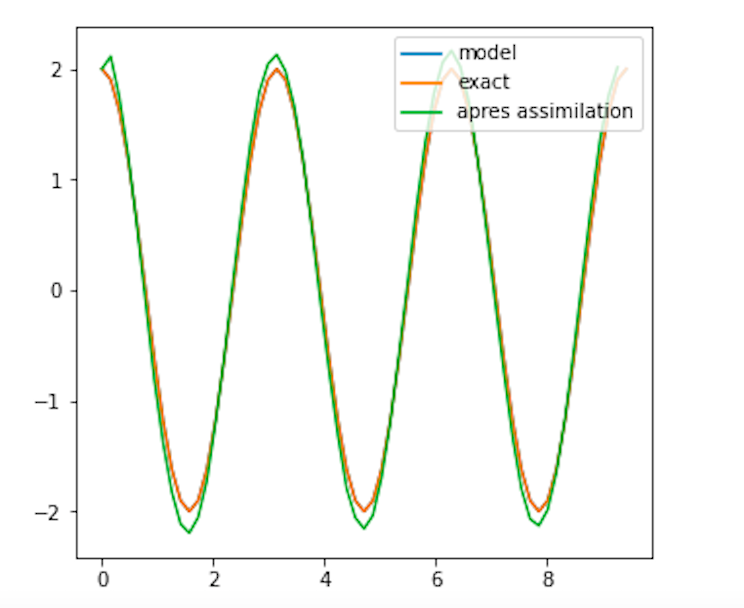
\includegraphics[width=0.4\textwidth]{"images/enkf/oscillator2.png"}
		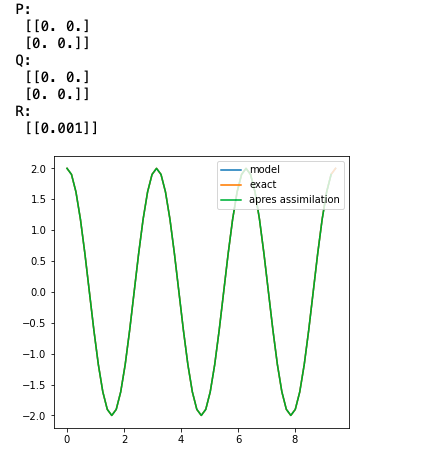
\includegraphics[width=0.4\textwidth]{"images/enkf/oscillator3.png"}
		\caption{Data assimilation with the harmonic oscillator}
\end{figure}
\noindent We have 3 different cases:
We tried to vary the covariance matrices associated with the error in order to understand their impact in the algorithm. For the first case we took a covariance matrix associated to the observation R smaller than the other matrices. This refers to the fact that our observations are very precise, they correspond to the exact solution. For Q, the covariance matrix associated to the model, we have also chosen an identity matrix, with in the diagonal the 0.1, since we solve it with the method of RK4 this one remains nevertheless quite accurate. And for P, in this case is a scalar because we observe only one component, and is equal to 0.1.
In the second case we have exactly the same value for R and Q, but we choose to take a  much bigger P than the one before to see if we have a difference. We can see that the green curve does not match exactly, it is much too far from our model and observation curve. This is because P represents the initial covariance matrix.
In the last case we choose to set the P and Q matrix to zero, so in fact we want to use the information from our model only, ignoring the observations. In this case we expect the curve after assimilation to be superimposed on the model curve, which is indeed the case. We will have that our $K=P^fH^T(HP^fH^T+R)^{-1}$ will be equal to 0.
\subsubsection{Lorenz system}
\noindent Now that we have tried the harmonic oscillator case, we can now look at the Lorenz system. The model will be the Lorenz system solved with RK4, and we will obtain our observations by solving the Lorenz system with different parameter values or different precision.
For the first case we chose to take exactly the same initial point and the same parameters for the observations and the model.
For $(\sigma, r, b)$ we have chosen to take (12.,6.,12.) and for the initial point we take (-10.,-10.,25.). But to differentiate the observations and the model we prefer to work with the time step. For the model we have chosen $dt=N/0.1$ and for the observations we have chosen $dt=N/0.01$ (with $N$ the number that represent the points of discretization). This means that, when we make the assimilation of the data  every 0.1 s., our observations will taken every 0.01 s.
\begin{figure}[H]
    \centering
		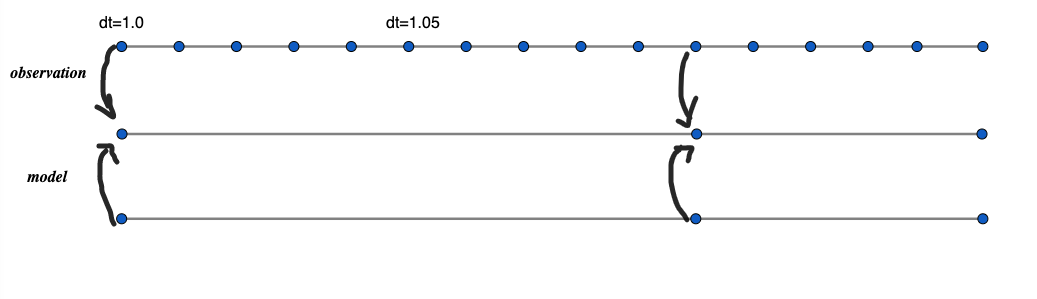
\includegraphics[width=1\textwidth]{"images/enkf/dt.png"}
		\caption{discretisation}
\end{figure}
We also chose to take a fairly small R because our observations are very precise.
\noindent\newline Let's take 
			$$P=\begin{pmatrix}
            0.1 & 0. & 0. \\
            0. & 0.1 & 0. \\
            0. & 0. & 0.1 \\
            \end{pmatrix} ,
            Q=\begin{pmatrix}
            0.1 & 0. & 0. \\
            0. & 0.1 & 0. \\
            0. & 0. & 0.1 \\
            \end{pmatrix},
            R=\begin{pmatrix}
            0.01 & 0. & 0. \\
            0. & 0.01 & 0. \\
            0. & 0. & 0.01 \\
            \end{pmatrix}.$$ 

\begin{figure}[H]
    \centering
		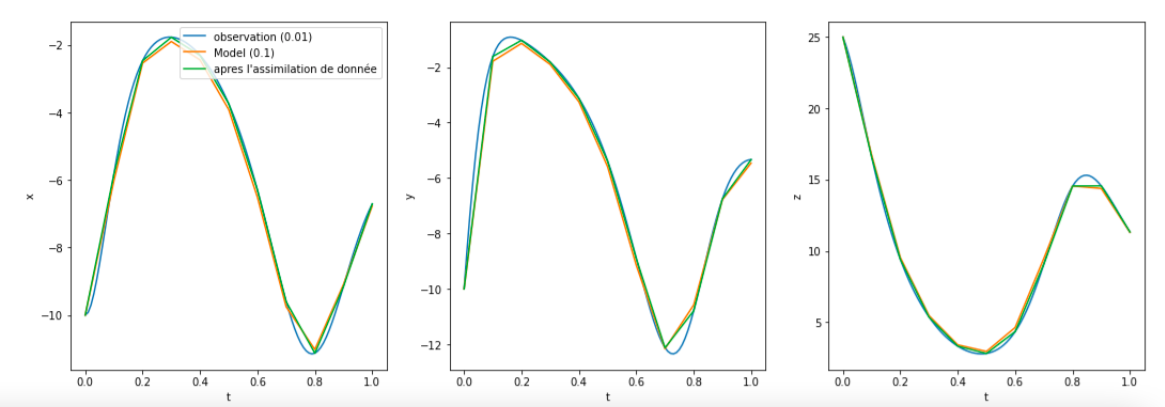
\includegraphics[width=1\textwidth]{"images/enkf/lorenz1_b.png"}
		\caption{First example for Lorenz with $(\sigma, r, b)=(12.,6.,12.)$, $X_0=(-10.,-10.,25.),\text{time step}=0.01s$ for observation and $0.1$s. for the model}
\end{figure}
\noindent We can notice that our curve after data assimilation is very close to our two other curves, we can see that our curve is very close to the model, which is totally normal, since we do the assimilation on each dt=N/0.1, it only takes the observations every 10 steps. But we can still see that the green curve is between the observations curve and the model curve.
\noindent \newline Let's try to change our parameters for the observations and the model. For $(\sigma, r, b)$ that we use in the observation we have chosen to take (12.,6.,12.), for the model $(\sigma, r, b)$=(10.,6.,10.) and for the initial point we take (-10.,-10.,25.) for both of them.
\noindent\newline Let's take 
			$$P=\begin{pmatrix}
            0.1 & 0. & 0. \\
            0. & 0.1 & 0. \\
            0. & 0. & 0.1 \\
            \end{pmatrix} ,
            Q=\begin{pmatrix}
            0.01 & 0. & 0. \\
            0. & 0.01 & 0. \\
            0. & 0. & 0.01 \\
            \end{pmatrix},
            R=\begin{pmatrix}
            0.1 & 0. & 0. \\
            0. & 0.1 & 0. \\
            0. & 0. & 0.1 \\
            \end{pmatrix}.$$ 
 \begin{figure}[H]
    \centering
		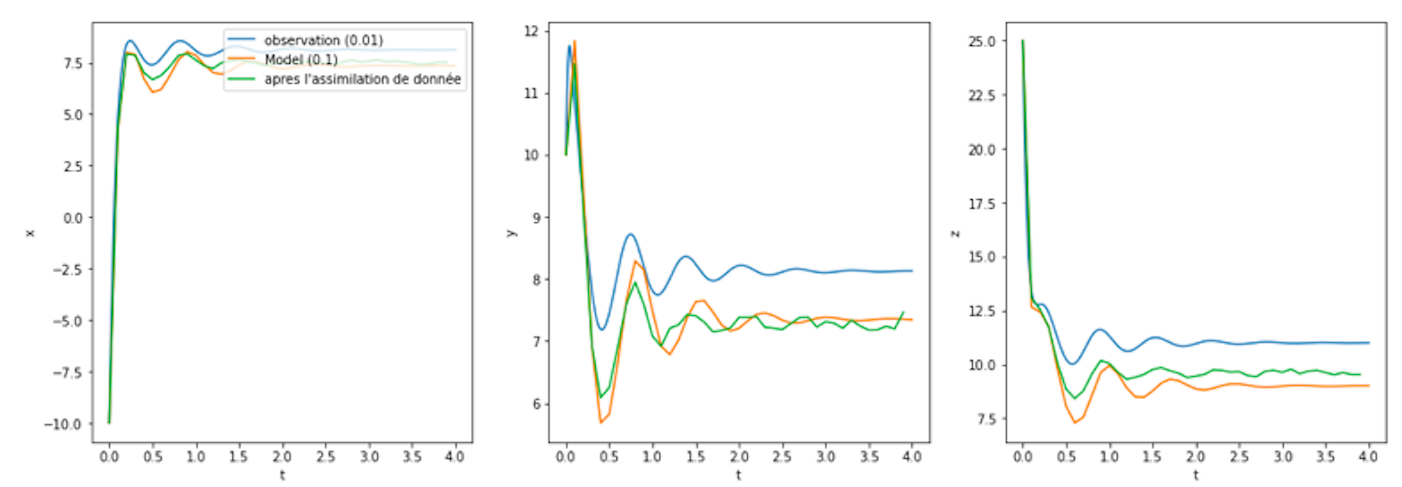
\includegraphics[width=1\textwidth]{"images/enkf/lorenz2_a.png"}
		\caption{Second example for Lorenz with $(\sigma, r, b)=(12.,6.,12.)$ for the observation, $(\sigma, r, b)=(10.,6.,10.)$ for the model, $X_0=(-10.,-10.,25.),\text{time step}=0.1s$ }
\end{figure}
\noindent This time we take a small Q, which means that we trust the model much more than the observations. We notice that our data assimilation curve is quite close to the one of the model, which confirms the assumptions we made when we chose Q and R.
\noindent\newline Let's take 
			$$P=\begin{pmatrix}
            0.1 & 0. & 0. \\
            0. & 0.1 & 0. \\
            0. & 0. & 0.1 \\
            \end{pmatrix} ,
            Q=\begin{pmatrix}
            0.1 & 0. & 0. \\
            0. & 0.1 & 0. \\
            0. & 0. & 0.1 \\
            \end{pmatrix},
            R=\begin{pmatrix}
            0.01 & 0. & 0. \\
            0. & 0.01 & 0. \\
            0. & 0. & 0.01 \\
            \end{pmatrix}.$$ 
 \begin{figure}[H]
        \centering
		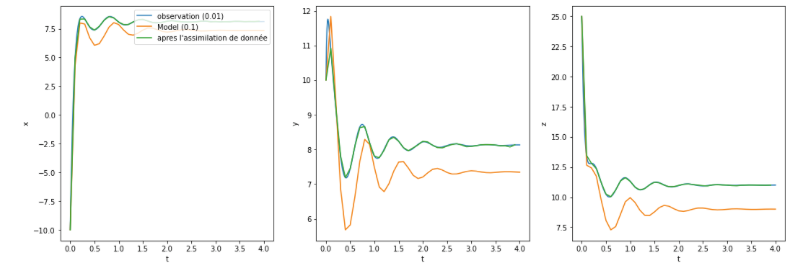
\includegraphics[width=1\textwidth]{"images/enkf/lorenz3_b.png"}
		\caption{Third example for Lorenz with $(\sigma, r, b)=(12.,6.,12.)$, $X_0=(-10.,-10.,25.),\text{time step}=0.01s$ for observation and $0.1$s. for the model}
\end{figure}
\noindent Now we have inverted the values of R and Q and we have not changed our P. We expect to see that our green curve is close to the blue curve which corresponds to the observations. On the other hand we notice that the values of the states after the data assimilation are very close almost similar to the observation ones.
